
\documentclass{article}
\usepackage{graphicx}
\usepackage{imakeidx}
\usepackage{geometry}
\usepackage{sectsty}
\geometry{
    left=1.5in,
    right=1in,
    top=1in,
    bottom=1.25in,
}





\title{\fontsize{16}{18}\selectfont\textbf{IOT PROJECT REPORT}\\[1em] \fontsize{14}{16}\selectfont\textbf{Project - Smart Agriculture System}\\[1em] \fontsize{12}{14}\selectfont\textbf{Modules - i) Smart Irrigation ii) Data Analytics}}
\author{\textbf{Assisted by}\\ Dr. E Suresh Babu \\[1em] \textbf{Performed by:}\\ R.Krishna 23CSM1R10 \\ V.Aashish Kumar 23CSM1S05}
\date{}

\begin{document}

\maketitle
\thispagestyle{empty} % Remove page number

\newpage





\tableofcontents % Generate table of contents

\newpage
\section{Introduction Smart Agriculture using IOT}
Smart Agriculture based on the Internet of things(IoT) completely changes the process of traditional agriculture methods and incorporates advanced technologies and integrates them to improve the process of agriculture significantly. On a practical level it uses smart devices like sensors,actuators and various other devices. These devices have the capabilities of monitoring the soil moisture, keeping an eye on temperature and humidity,and observing the crop health on a regular basis. They are also capable of automating manual processes like supplying water to crops based on requirement. With the help of incorporating these devices into farming, farmers can make efficient decisions and optimize resources which ultimately results in improving the crop yield. Incorporating IoT aspects into agriculture not only helps farmers but also contributes to sustainable environmental development by efficient usage of natural resources without wastage. It makes farming easier and efficient for farmers and helps the environment by efficient utilization of resources. Incorporating intelligent devices, real time data collection and taking intelligent decisions based on data collected can make agriculture much more easy and effective
		Amongst many research domains on introducing IoT in agriculture systems, we mainly focus on 2 important aspects\\
	→Smart Irrigation\\
	→Data Analytics



\subsection{Introduction to Smart Irrigation system }
Smart irrigation system is an effective idea of managing water in crop fields in a smarter way. It makes use of technology and incorporates intelligent devices such as sensors and actuators along with communication devices to make the irrigation process in a more sustainable way. A smart irrigation system works by continuously monitoring some factors such as soil moisture, temperature, humidity and weather conditions in real time and take appropriate actions accordingly.

\subsection*{Illustration with use case : smart irrigation in Apple farm}
In an apple farm, maintaining the appropriate moisture level in soil is very important for the huge productivity of apple trees. To maintain the appropriate moisture level, soil moisture sensors are strategically placed in the apple farm. When the uncertainty is detected by the sensors, the smart irrigation system is notified and the smart irrigation system delivers water at the appropriate zone which ensures healthy productivity.We can also dynamically adjust the irrigation process based on climatic conditions.This makes sure that over watering and underwater irrigation cannot happen ultimately giving us better results. Smart irrigation not only conserves water but also improves the crop health and ultimately increases the yield.
\subsection{Data Analytics- Overview}
Data analytics plays an extensive role in smart agriculture by providing useful information and meaningful perspectives from the data. It helps farmers in effective decision making and strategic moves. It kind of revolutionaries traditional farming practices by leveraging real time data. 	We can summarize the data analytics process in the following steps.

\begin{itemize}
    \item \textbf{Data Collection} Data collection can be done by making use of sensors and they collect data related to soil conditions, temperature,humidity, crop health.


    
    \item \textbf{Processing of data
}  It involves transformation of data into meaningful information from the raw form. It can include the tasks like cleaning the data, validating the data, handling missing values in the data and performing statistical analysis on the data.
    
    \item \textbf{Data integration} Combining the data from different sources into a clear view. It involves adding data from various sources and creates a unified dataset providing a full picture. It facilitates more accurate and holistic analysis and enables decision making to be done in an effective way.

     \item \textbf{Performing analytics} On the collected and processed data we can perform predictive analysis to forecast events like crop yield and perspective analytics to offer recommendations for efficient farming.

      \item \textbf{Decision support and resource optimization} Data analytics gives farmers the insights into the data and leads them to make good decisions and it leads to effective resource utilization.
\end{itemize}

    \section{Types of Sensors Used (For Implementation of This Project in the Physical World)}
\begin{enumerate}
    \item \textbf{Soil Moisture Sensors:}
    \begin{itemize}
        \item \textbf{Functionality:} Moisture content measurement in soil.
        \item \textbf{Reason for Using:} If we know the moisture content of soil, we can determine when and how much water is required by soil, preventing cases like underwatering and overwatering.
    \end{itemize}
    
    \item \textbf{Temperature Sensors:}
    \begin{itemize}
        \item \textbf{Functionality:} Measure the temperature level of air and soil.
        \item \textbf{Reason for Using:} Temperature conditions majorly affect plant growth, and knowing the temperature in real-time can help make appropriate decisions regarding providing water to the crop.
    \end{itemize}
    
   
    
    \item \textbf{Solar Radiation Sensors:}
    \begin{itemize}
        \item \textbf{Functionality:} Measure the amount of sunlight received.
        \item \textbf{Reason for Using:} Crop growth is affected by evaporation rates, and evaporation rates are influenced by sunlight received. Acquiring solar data can be used to adjust irrigation schedules accordingly.
    \end{itemize}
    
    \item \textbf{pH Sensors:}
    \begin{itemize}
        \item \textbf{Purpose:} Measurement of the volume of water used.
        \item \textbf{Reason for Using:} Soil pH affects nutrient availability for plants. Knowing the pH details helps perform irrigation better.
    \end{itemize}
    
    
\end{enumerate}

\section{Virtualization Infrasturcture Components}
To illustrate the above sensors virtually we can take any simulation platforms that replicate the behavior of physical sensors digitally. Initially we have to identify the sensors we require and design the virtual environment for these sensors. We have to appropriately specify the characteristics of these sensors. We next have to integrate these virtual sensors with the IoT platform for data management and analysis. It is a cost effective means of prototype which enables physical architecture into virtual systems. 

\subsection{Software Requirements}
In the process of implementing the smart agriculture system, we use the following simulation software and Integrated Development Environments(IDEs):

\begin{itemize}
    \item \textbf{My understanding of Contiki-NG:}
    Our understanding of Contiki-NG: Designed specifically for Internet of Things (IoT) devices, Contiki-NG is an open-source operating system that can run on devices with low memory and processing power. Contiki-NG is used in this project to build an actuator and sensor network that is networked and to simulate Internet of Things devices. These devices collect essential data about soil moisture content, ambient conditions, and other agriculturally relevant characteristics.
\end{itemize}

\begin{itemize}
    \item \textbf{My understanding of Cooja Simulator}
    
COOJA(Contiki network simulator) is a network simulator designed for Internet Of Things(IoT) and Wireless Sensor Networks(WSN). Cooja allows to simulate large scale networks of sensor nodes and performance evaluation can be done under various conditions. It provides virtual environment which is similar to physical hardware. 
Whatever the applications developed by us in Contiki based environment, with the help of cooja simulator is to test and debug our Contiki based applications. Cooja supports IEEE 802.15.4,6LoWPAN and CoAP kind of protocols.

\end{itemize}
\begin{itemize}
    \item \textbf{My understanding of Jupyter notebook}
    
It is an open source web application by which we can create and share python projects. It can even have support for programming languages like R,Julia. In our project we used jupyter notebook to create crop recommendation system and smart irrigation system modules. Jupyter notebooks can easily allow for collaboration and reproducibility.

\end{itemize}

\begin{itemize}
    \item \textbf{My understanding of Spyder}
    
Spyder is an Integrated Development Environment(IDE) used for data analysis in python. It provides various tools needed for data scientists and engineers. Spyder supports several numerical libraries like pandas,numpy,SciPy which are used in data manipulation and numerical computation. In our project we utilized spyder to construct interactive and visually engaging  web-based interface. We were able to design the dashboard by leveraging spyder's capabilities
\end{itemize}


\newpage
\section{System Architecture} 

\begin{figure}[h]
    \centering
    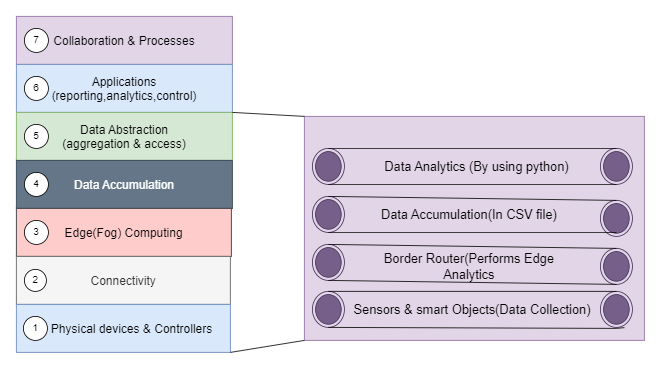
\includegraphics[width=1.0\textwidth]{IWF_IOT_Architecture.drawio (2)}
    \caption{IWF  IOT  Architecture}
    \label{fig:example}

    \centering
    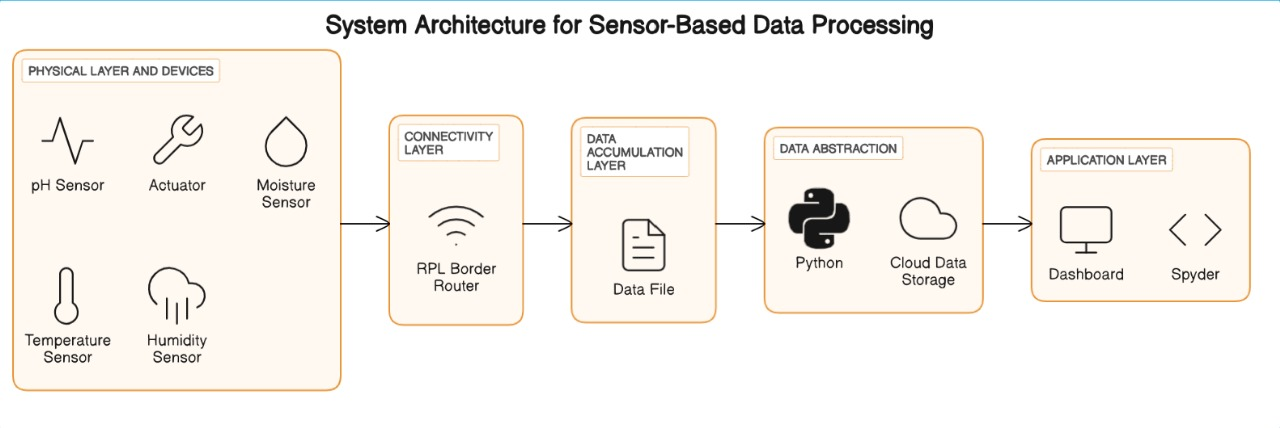
\includegraphics[width=1.0\textwidth, height=2in]{system_architecture.jpg}  
    \caption{system architecture}
    \label{fig:example}
\end{figure}
IWF(IoT workflow) architecture is the reference of structure designed for IoT system. The group of tasks are divided into several layers where each layers encapsulates the particular functionalities. The architecture clearly explains which task is being performed at which state.
\newpage
\section{Methodology}
\begin{figure}[h]
    \centering
    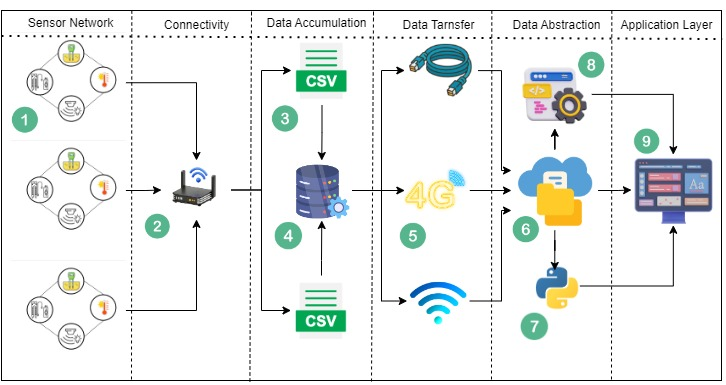
\includegraphics[width=1\linewidth]{dataflow1.jpg}
    \caption{Data Flow}
    \label{fig:enter-label}
\end{figure}

\begin{itemize}
    \item Step 1: Data generated by various, integrated sensors.
    \item Step 2: Generated data from various sensor networks is collected by border router.
    \item Step 3: Storage of data generated by sensors in different CSV files by border router.
    \item Step 4: Data is aggregated in local database from CSV files.
    \item Step 5: The aggregated data is sent to central cloud storage by different networking technologies.
    \item Step 6: The data gets stored in cloud storage.
    \item Step 7: Python program uses data to analyze the generated data and perform different machine learning techniques and visualizations.
    \item Step 8: Based on machine learning tasks performed, Spyder software is used to develop an interactive dashboard to show various results.
    \item Step 9: The results of performed machine learning algorithms are shown in the dashboard.
\end{itemize}

\section{Comprehensive Theoretical Framework}

\subsection{Physical devices and controllers}

In our smart agriculture project as a part of smart irrigation module we are using several physical devices and controllers which are meant to monitor irrigation process efficiently. We use several sensors intended to do required smart work and these sensors are integrated with centralized controller whose job is to process the data and adjust the irrigation parameters based on predefined threshold values. Altogether they provide an intelligent irrigation system capable of increasing the productivity.
\subsection*{Different kinds of sensors}

\begin{enumerate}
    \item \textbf{Soil Moisture Sensors}: 
    
    \item \textbf{pH sensors}: 
    
    \item \textbf{Temperature sensor}: 
    \item \textbf{Light sensors}:
\end{enumerate}

\textbf{Sky Mote}: This particular mote integrates all above-mentioned sensors crucial for monitoring environmental conditions.

\subsection{Connectivity}
\maketitle

In our smart agriculture project, 6LoWPAN connectivity mechanism between sky mote sensor nodes, gateway nodes, and other components of the IoT network. We can achieve data transmission efficiently and interoperability seamlessly by using this communication protocol. 

\subsection{Edge computing}

To implement edge computing in our project we followed the following steps:

\begin{enumerate}
    \item \textbf{Data Aggregation and Preprocessing}: Initially, the border router can be configured to collect sensor data from sky mote sensor nodes deployed in the field. The collected sensor data can be aggregated over a specified time interval to reduce the volume of data transmitted to the edge devices.
    
    \item \textbf{Setup}: We have considered the border router as an edge device for the data processing to be done at the edge level.
    
    \item \textbf{Data processing and analysis}: The aggregated sensor data from the border router can be used to perform edge computing tasks. Among the obtained data, we can implement real-time data analysis and anomaly detection for predictive modeling.
\end{enumerate}

\subsection{Data Accumulation}

\begin{enumerate}
    \item \textbf{Data storage}: To store our data we have chosen Google Sheets which is a file-based storage solution.
    
    \item \textbf{Data accumulation logic}: On the edge device, we can accumulate processed sensor data over time intervals. A Python code can be helpful to do that task, and we can continuously receive, process, and store sensor data in the chosen storage solution (Google Sheets in our case).
    
    \item \textbf{Integration with data analytics}: A seamless integration between data accumulation and data analytics is done here.
\end{enumerate}

\subsection{Data abstraction}

In the process of data abstraction, we have used several data models which are mentioned as:

\begin{enumerate}
    \item \textbf{Data visualization}: The modules leverage abstracted sensor data to create insights. We have used Python libraries like Matplotlib, Seaborn to generate several types of visualizations. The different visualizations we have considered are line charts, scatter plots, and histograms.
    
    \item \textbf{Smart irrigation}: The module takes moisture and temperature as inputs and informs whether to turn off or turn on the motor which helps farmers to take instantaneous decisions about giving water to plants.
    
    \item \textbf{Crop recommendation system}: This module takes seven parameters such as nitrogen level, phosphorus level, potassium level, temperature, rainfall, humidity, and moisture level to recommend the appropriate crop. Based on values generated by sensors, we applied a deep learning model using Artificial Neural Networks to recommend the best crop.
\end{enumerate}

\subsection{Application}

This entire data analytics part containing three modules is shown as one web application which allows us to select the appropriate module:

\begin{enumerate}
    \item \textbf{Data visualization module}: Shows different types of graphs to understand the data visually.
    
    \item \textbf{Smart irrigation system}: Allows users to enter moisture and temperature values and shows a message whether to turn off or turn on the motor.
    
    \item \textbf{Crop recommendation system}: Allows users to enter seven values and recommend the best crop according to appropriate conditions.
\end{enumerate}










\section{Implementation } 
In the process of implementation, we learned the use of the required tools and we started learning how to use them.
\subsection{Installation of Contiki-ng }
We have installed contiki-ng on a vmware virtual machine.Later we created a sensor as per our project requirement.

\subsection{Sensor setup}
We created 3 virtual networks of sensors and connected them to the rpl border router. Each sensor generates values of ph,temperature,humidity and light intensity. Those values are accumulated at border router which acts as a connectivity level between physical devices and cloud part.
In the implementation border router is used to to send and receive messages so border router is implemented.
\begin{figure}[ht]
    \centering
    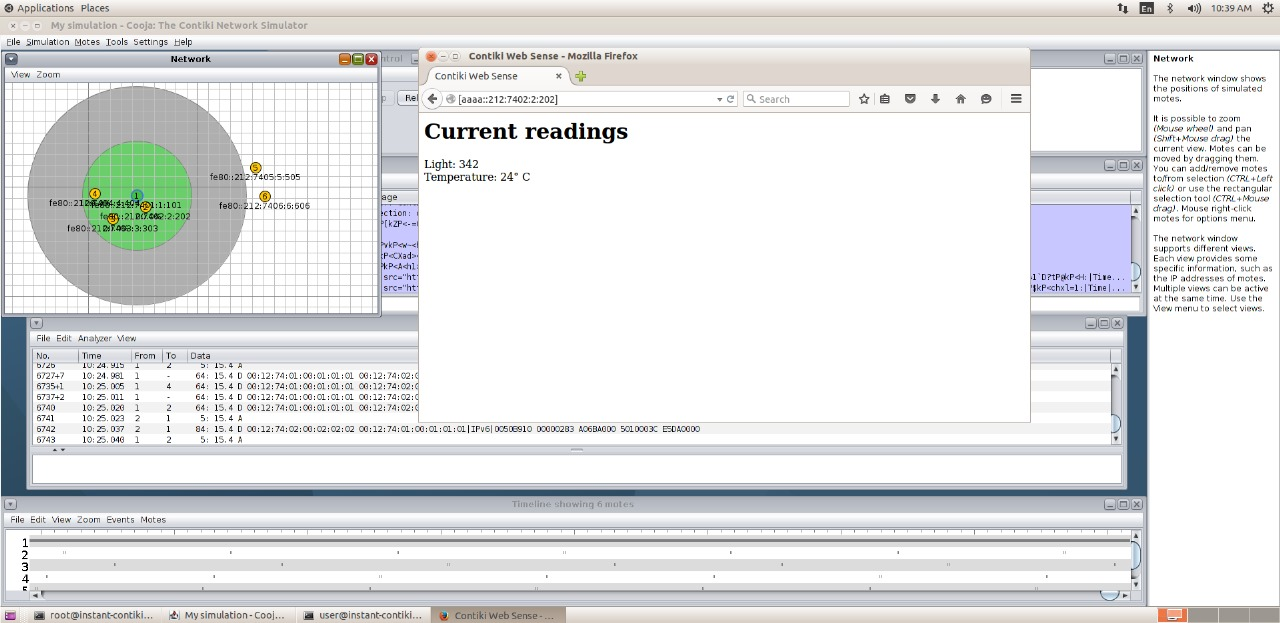
\includegraphics[width=1.0\textwidth]{contiki pic 2.jpg}
    \caption{Sensor setup}
    \label{fig:example}
\end{figure}


\subsection{Border router connection & storage}
Whenever we have given appropriate ip address of sensors, those generated values are being displayed. It specifies that border router is connected to the internet.
Now along with printing the values we can save those values in a text file by leveraging the functionality of c programming language. So whenever the value is being displayed, it is automatically stored in the text file. 
\subsection{Convertion of text file to csv file}
For the data analytics part, we can convert generated text file into csv file which contains comma separated values of different sensor values.
Now the generated csv file is stored in cloud fo further analysis.
\newpage
\subsection{Data Analytics}
Based on data generated by the sensors(which is stored in csv file), we have implemented several tasks related to data analytics.
\begin{figure}[h]
    \centering
    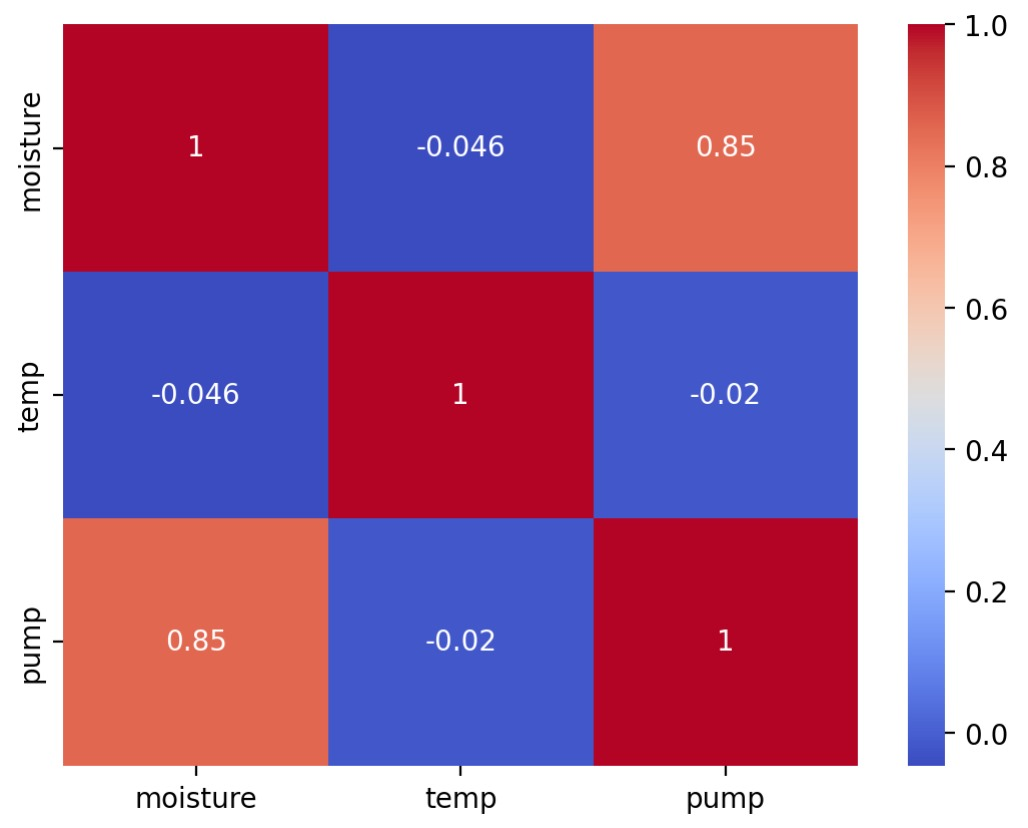
\includegraphics[width=0.75\linewidth, height=2.5in]{dataanalytics.jpg}
    \caption{Enter Caption}
    \label{fig:enter-label}
\end{figure}
\newpage
\subsubsection{Dashboard Home page: }

Based on sensor generated data various operations can be performed by the help of various machine learning and deep learning algorithms. We can even represent data in various visualization forms by different pictorial representations. \\
For our project we majorly consider 4 modules named 
\begin{itemize}
    \item 1: Smart Irrigation
    \item 2: Crop Prediction
    \item 3: Analysis
    \item 4: Data Genration
\end{itemize}
\\
\\
\begin{figure}[h]
    \centering
    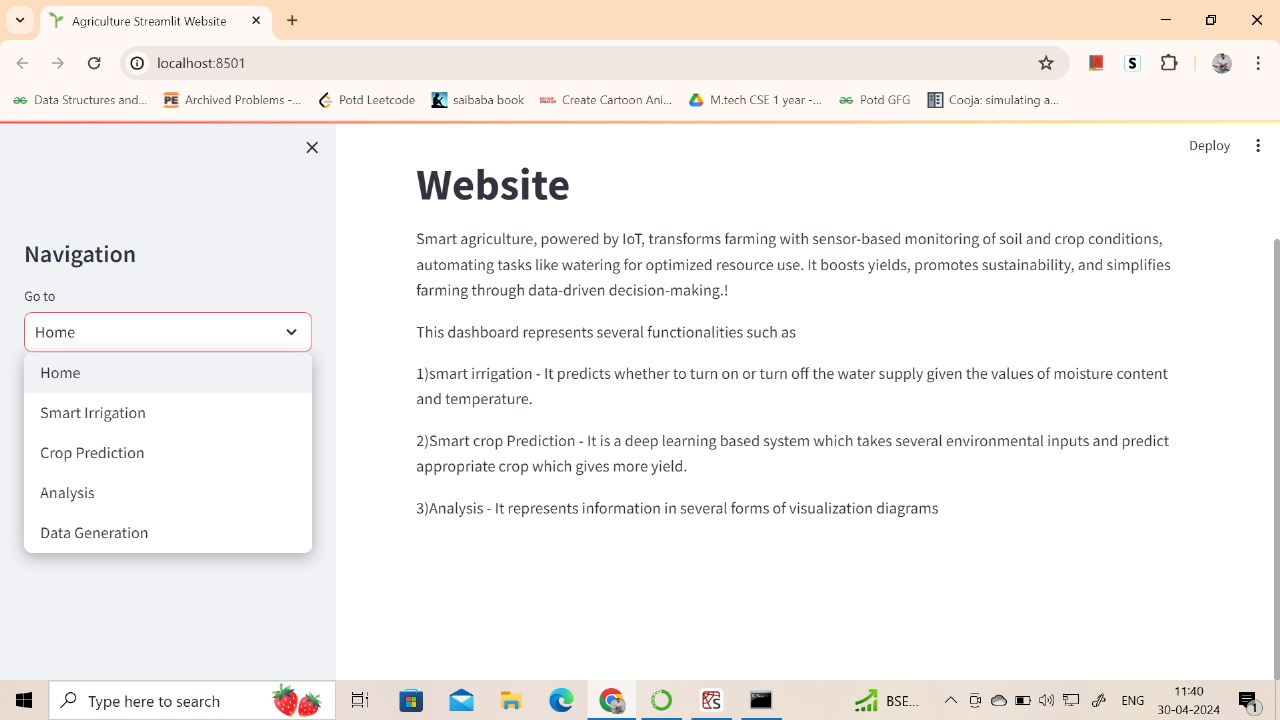
\includegraphics[width=1.0\textwidth]{Dashboard_Home.jpg}
     
    \caption{Dashboard Home }
    \label{fig:example}
\end{figure}
\newpage
\subsubsection{Data generation: }

Purpose : The generated data by the sensors in contiki platform are being shown here \\
Implementation: As we are storing sensor generated data in a file and file is being uploaded to cloud. To implement this particular module that file values are taken into consideration, and data is being displayed.
\\
\\
\begin{figure}[h]
    \centering
    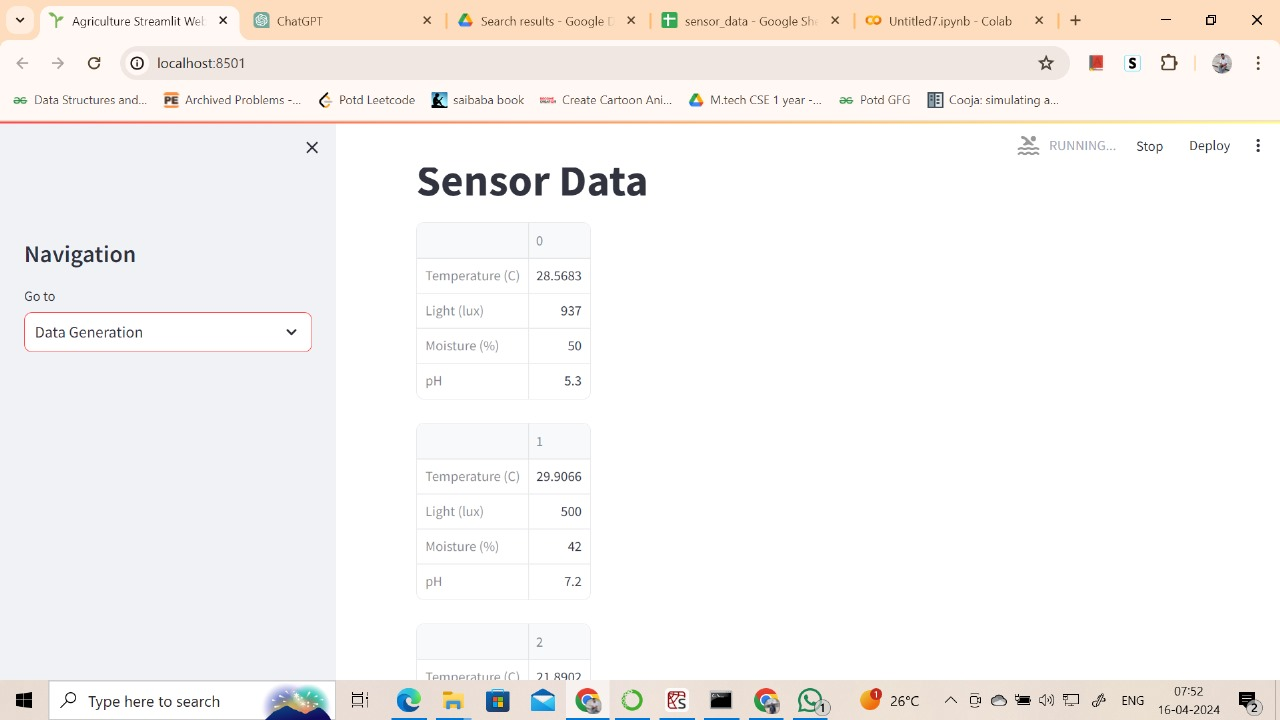
\includegraphics[width=1.0\textwidth]{Data_generation.jpg}
     
    \caption{Data Generation}
    \label{fig:example}
\end{figure}
\newpage
\subsubsection{Smart irrigation:}

Purpose : It predicts whether to turn on or turn off the water supply given the values of moisture content and temperature.\\
Implementation : We trained a machine learning model by taking motor pump dataset and used artificial neural networks to train our model based on specified dataset. After the model being trained, If we give values generated by our sensors, particularly temperature and moisture , model will predict whether to turn on or turn off the motor. 
\\
\\
\begin{figure}[h]
    \centering
    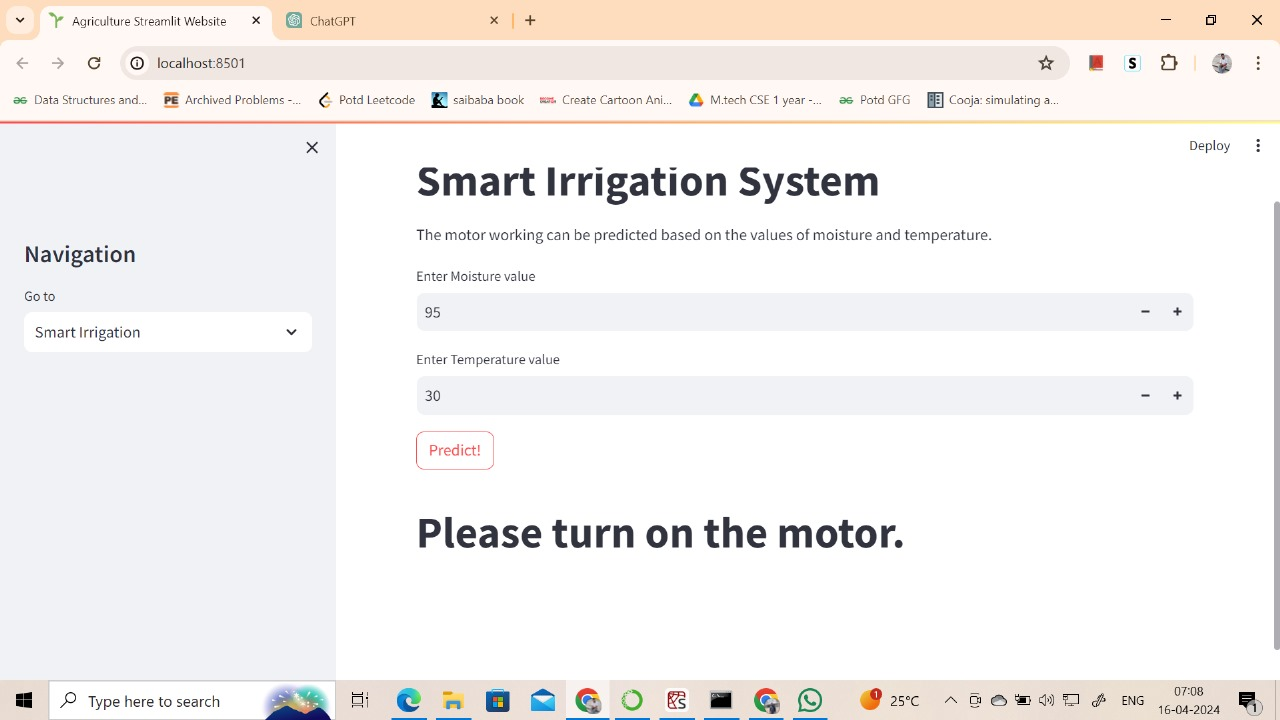
\includegraphics[width=1.0\textwidth]{smart_irrigation_system.jpg}
    \caption{Smart Irrigation System}
    \label{fig:example}
\end{figure}
\newpage
\subsubsection{Smart Crop Prediction}

\textbf{Purpose:} It is a machine learning-based system that takes several environmental inputs and predicts the appropriate crop that gives more yield.\\
\textbf{Implementation:} We trained a machine learning model using a crop prediction dataset with artificial neural networks algorithm. Our model takes inputs such as Nitrogen value, Phosphorus value, Potassium value, temperature, and humidity. It predicts the best crop appropriate to the given conditions. We tested our model with values generated by our sensors.

\begin{figure}[h]
    \centering
    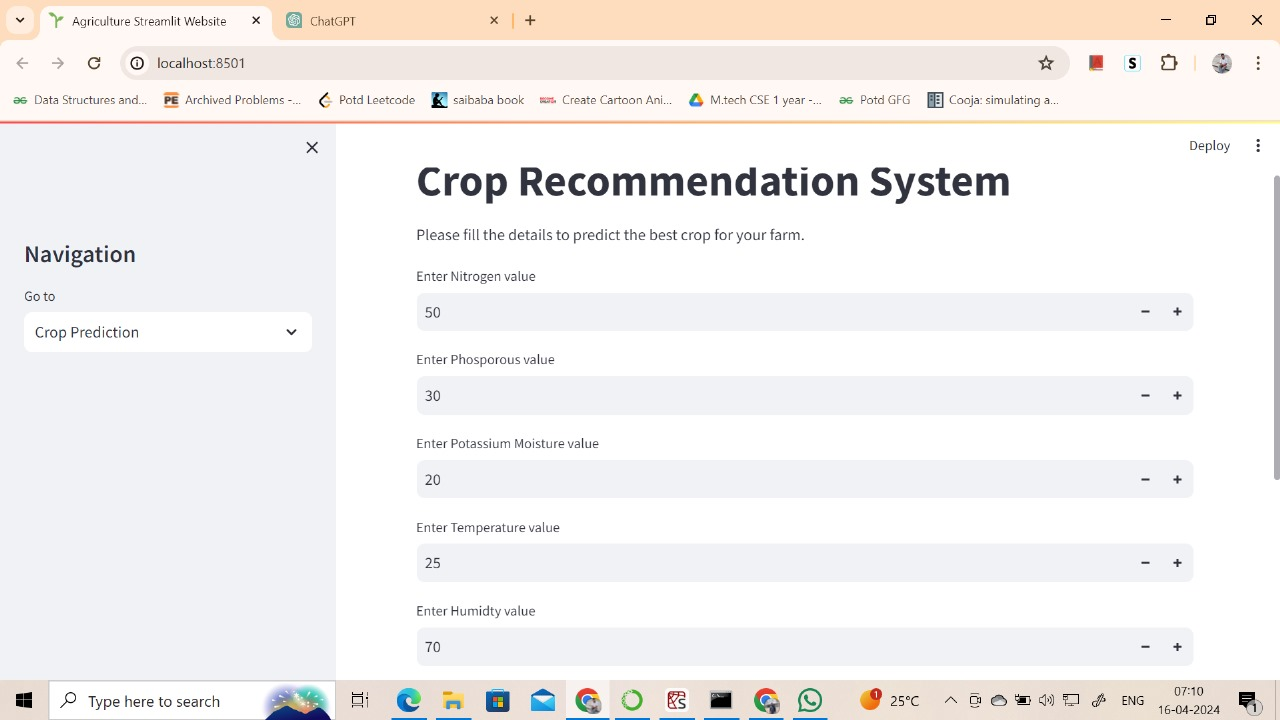
\includegraphics[width=0.8\textwidth]{crop_recommendation_system.jpg}
    \caption{Crop recommendation system parameters}
    \label{fig:example1}
\end{figure}

\begin{figure}[h]
    \centering
    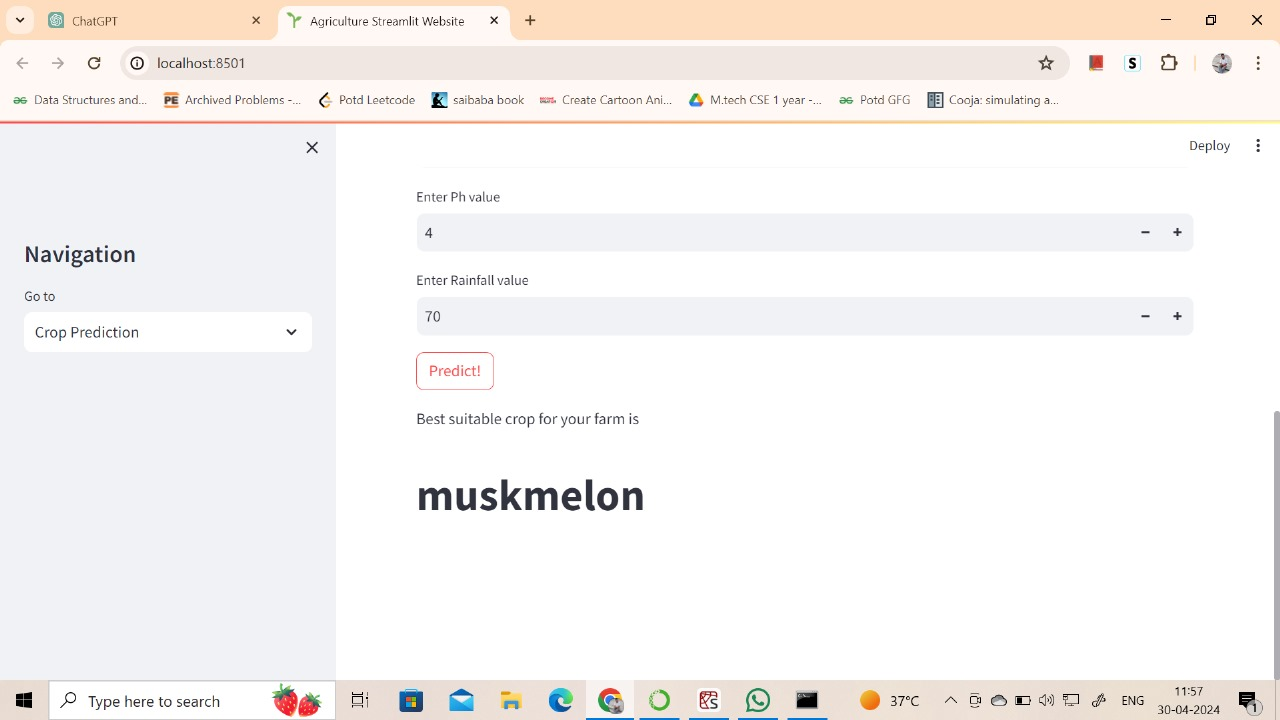
\includegraphics[width=0.8\textwidth]{crop_recommendation_system1.jpg}
    \caption{Crop recommendation system results}
    \label{fig:example2}
\end{figure}

\newpage



\subsubsection{Analysis & Visualization }
 
Purpose:It represents information in several forms of visualization diagrams.\\
Implementation: Based on generated data we pictorially represented information in the form of bar charts and histogram for visualization purpose of information.
\\

\begin{figure}[h]
    \centering
    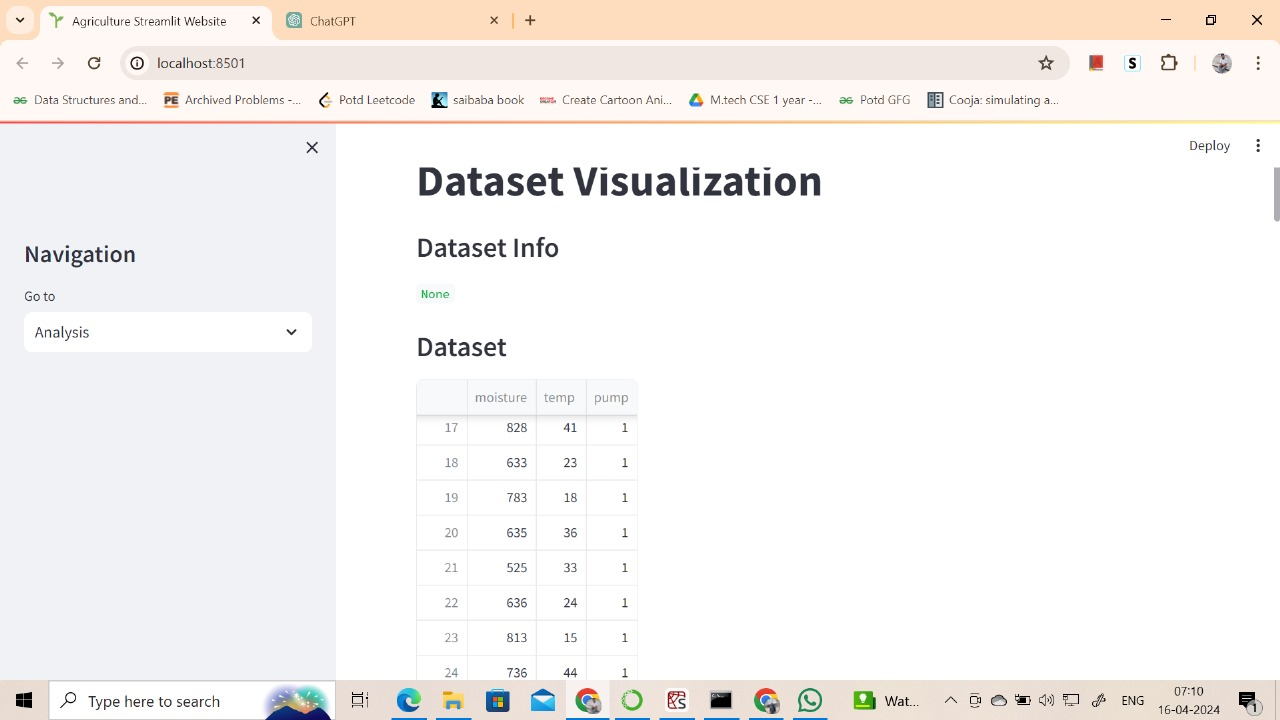
\includegraphics[width=0.8\textwidth]{dataset_visualization.jpg}
    \caption{Data Representation}
    \label{fig:example}
\end{figure}

\begin{figure}[h]
    \centering
    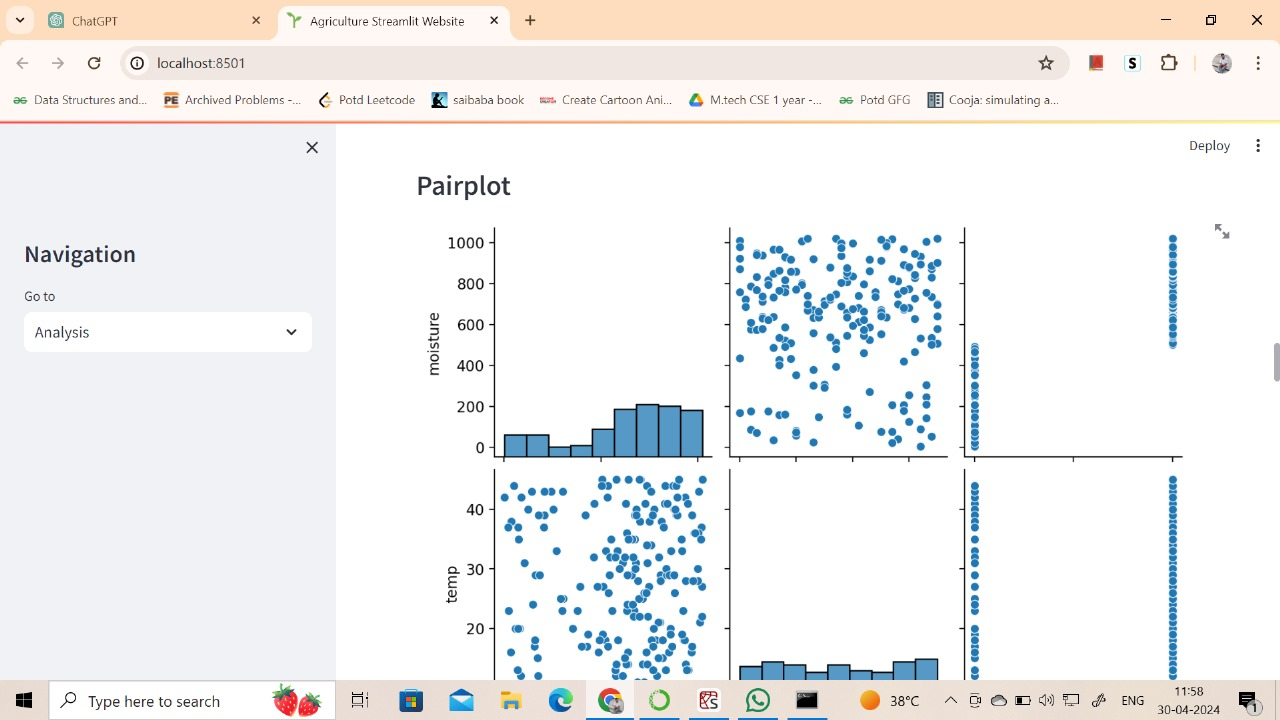
\includegraphics[width=0.8\textwidth]{dataset_visualization1.jpg}
    \caption{Dataset visualization }
    \label{fig:example}
\end{figure}

\begin{figure}[h]
    \centering
    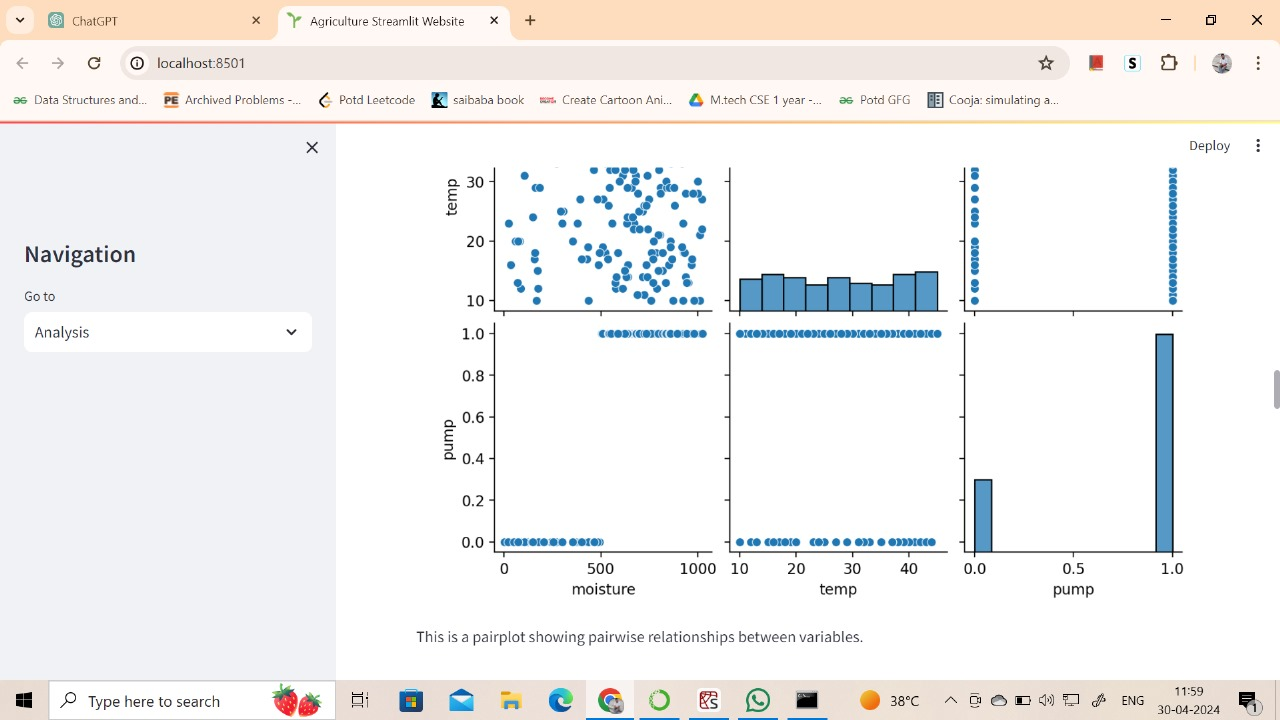
\includegraphics[width=1.0\textwidth]{dataset_visualization2.jpg}
    \caption{Dataset Visualization}
    \label{fig:example}
\end{figure}
\newpage

\section{Conclusion}

The implementation of Smart irrigation and data analytics modules by leveraging the concepts of Internet of Things and Machine learning algorithms can revolutionaries the idea of traditional farming and paves the way for precision farming based framework. It actually makes farming more easy. It helps the farmers to optimize and efficiently utilize the resources to make informed decisions. Adoption of IoT concepts in smart agriculture not only improves the efficiency but also leads to sustainable farming. Overall the incorporation of intelligent devices in real time environment strengthens agriculture ecosystem.

\end{document}


